% Created 2012-12-10 Mon 12:28
\documentclass[11pt]{article}
\usepackage[utf8]{inputenc}
\usepackage{fixltx2e}
\usepackage{url}
\usepackage{graphicx}
\usepackage{minted}
\usepackage{color}
\usepackage{longtable}
\usepackage{float}
\usepackage{wrapfig}
\usepackage{soul}
\usepackage{textcomp}
\usepackage{amsmath}
\usepackage{marvosym}
\usepackage{wasysym}
\usepackage{latexsym}
\usepackage{amssymb}
\usepackage[linktocpage,
  pdfstartview=FitH,
  colorlinks,
  linkcolor=blue,
  anchorcolor=blue,
  citecolor=blue,
  filecolor=blue,
  menucolor=blue,
  urlcolor=blue]{hyperref}
\usepackage{attachfile}
\tolerance=1000
\providecommand{\alert}[1]{\textbf{#1}}

\title{Final Project Report}
\author{Yichun Sun}
\date{2012-12-10 Mon}
\hypersetup{
  pdfkeywords={},
  pdfsubject={},
  pdfcreator={Emacs Org-mode version N/A-fixup}}

\begin{document}

\maketitle

\setcounter{tocdepth}{3}
\tableofcontents
\vspace*{1cm}

\section{Objective}
\label{sec-1}

This project is to calculate different adsorption energy of oxygen on different surface sites of different transition metals and estimate oxygen diffusion barrier.
\section{Existed work on this problem}
\label{sec-2}

\begin{enumerate}
\item S Yamagishi, S.J Jenkins and D.A King calculated O on Ni(111), concluded that the adsorption energy for fcc,hcp and bridge sites were -4.21, -4.05 and -3.14 eV/O2, estimated the diffusion barrier was between 0.46 and 0.54 eV.
   Link: \href{http://dx.doi.org/10.1016/j.susc.2003.08.002}{http://dx.doi.org/10.1016/j.susc.2003.08.002}
\item Mira Todorova, Karsten Reuter, and Matthias Scheffler calculated the oxygen adsorption energy on Pd(111), which were -1.5 and -1.2 eV/O for fcc and hcp.
   Link: \href{http://dx.doi.org/10.1021/jp040088t}{http://dx.doi.org/10.1021/jp040088t}
\item April D. Daigle, Joseph J. BelBruno calculated the oxygen adsorption energy on Au(111). The result were -3.38, -3.15 and -3.05 for fcc, hcp and bridge sites respectively.
   Link: \href{http://dx.doi.org/10.1016/j.susc.2011.04.025}{http://dx.doi.org/10.1016/j.susc.2011.04.025}
\item Aloysius Soon, Mira Todorova,et al calculated the oxygen adsorption energy on Cu(111) and found it was -1.65 eV at 0.25ML coverage.
   Link: \href{http://dx.doi.org/10.1103/PhysRevB.73.165424}{http://dx.doi.org/10.1103/PhysRevB.73.165424}
\item In DFT BOOK, Prof. Kitchin calculated the oxygen adsorption on Pt(111).
\end{enumerate}
\section{Method}
\label{sec-3}
\subsection{Definition of adsorption energy}
\label{sec-3-1}


$\Delta H_{ads} (eV/O) = E_{slab+O} - E_{slab} - 0.5*E_{O_2}$

I assume the oxygen molecule has split in half, and that the atoms have moved far apart. I choose the oxygen coverage at 0.25ML. For computational speed, the slab is frozen but the adsorbate is relaxed.
\subsection{convergence study}
\label{sec-3-2}
\subsubsection{cutoff energy convergence}
\label{sec-3-2-1}

Here i will give 2 examples, the rest are similar.
\begin{itemize}

\item O2\\
\label{sec-3-2-1-1}%
\begin{minted}[frame=lines,fontsize=\scriptsize,linenos]{python}
from jasp import *
from ase import Atom, Atoms
encuts = [250, 300, 350, 400, 450, 500, 550]

D = []
for encut in encuts:
    atoms = Atoms([Atom('O', [5,    5, 5], magmom=1),
                   Atom('O', [6.22, 5, 5], magmom=1)],
              cell=(10,10,10))

    with jasp('convergence/O2/convergence-{0}'.format(encut),
              xc='PBE',
              encut=encut,
              ismear=0,
              ispin=2,  # turn spin-polarization on
              ibrion=2, # this turns relaxation on
              nsw=10,
              atoms=atoms) as calc:
        try:
            E_O2 = atoms.get_potential_energy()
        except (VaspSubmitted, VaspQueued):
            E_O2 = None

        D.append(E_O2)

import matplotlib.pyplot as plt
plt.plot(encuts, D)
plt.xlabel('ENCUT (eV)')
plt.ylabel('O$_2$ potential energy (eV)')
plt.savefig('images/convergence/O2-convergence.png')
plt.show()
\end{minted}

\begin{verbatim}
 None
\end{verbatim}
\begin{figure}[H]
\centering
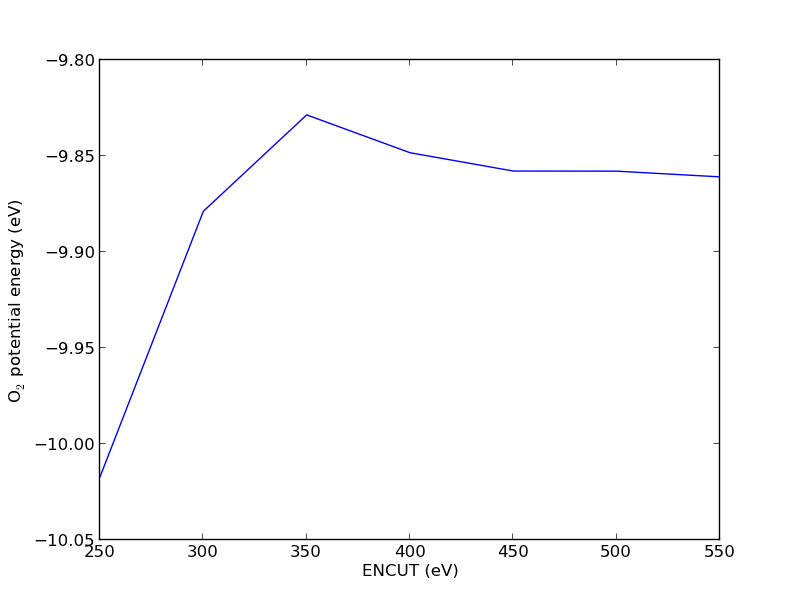
\includegraphics[width=0.7\textwidth]{./images/convergence/O2-convergence.png}
\caption{Oxygen cutoff energy convergence}
\end{figure}

So I choose encut= 400 eV for O$_2$ potential energy.


\item Ni\\
\label{sec-3-2-1-2}%
\begin{minted}[frame=lines,fontsize=\scriptsize,linenos]{python}
from jasp import *
from ase.lattice.surface import fcc111
from ase.constraints import FixAtoms
encuts = [250, 300, 350, 400, 450, 500, 550]

D=[]
for encut in encuts:
   atoms = fcc111('Ni', size=(2,2,3), vacuum=10.0)
   constraint = FixAtoms(mask=[True for atom in atoms])
   atoms.set_constraint(constraint)

   with jasp('convergence/Ni/Convergence-e-{0}'.format(encut),
          xc='PBE',
          kpts=(4,4,1),
          encut=encut,
          atoms=atoms) as calc:
    try:
       slab_e = atoms.get_potential_energy()
    except (VaspSubmitted,VaspQueued):
       slab_e=None

    D.append(slab_e)
import matplotlib.pyplot as plt
plt.plot(encuts,D)
plt.xlabel('ENCUT (eV)')
plt.ylabel('Ni slab energy (eV)')
plt.savefig('images/convergence/Ni_encut_convergence.png')
plt.show()
\end{minted}

\begin{verbatim}
 None
\end{verbatim}
\begin{figure}[H]
\centering
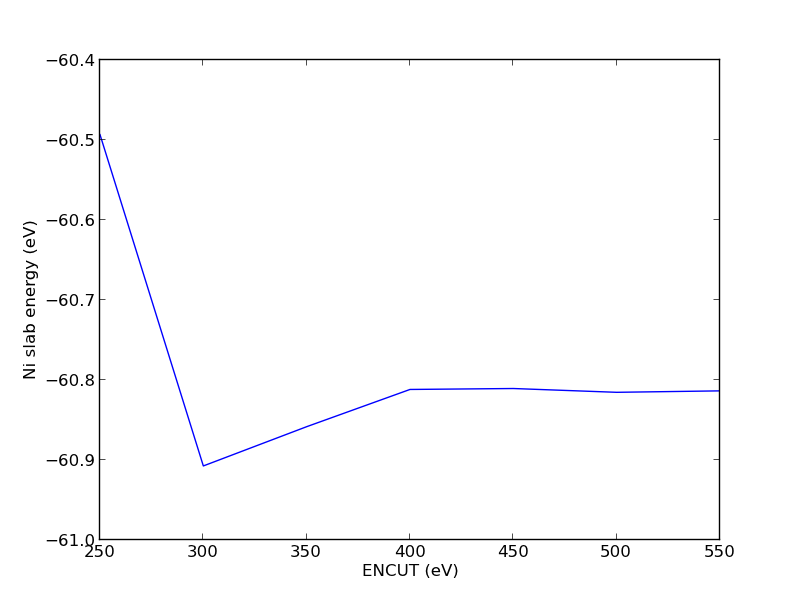
\includegraphics[width=0.7\textwidth]{./images/convergence/Ni_encut_convergence.png}
\caption{Ni cutoff energy convergence}
\end{figure}

We choose encut = 400eV.

\end{itemize} % ends low level
\subsubsection{k-point convergence}
\label{sec-3-2-2}

Here I will give an example of Ni, the rest metals are similar.

\begin{minted}[frame=lines,fontsize=\scriptsize,linenos]{python}
from jasp import *
from ase.lattice.surface import fcc111
from ase.constraints import FixAtoms
KPTS = [2,3,4,5,6,8,10]

D=[]
for k in KPTS:
   atoms = fcc111('Ni', size=(2,2,3), vacuum=10.0)
   constraint = FixAtoms(mask=[True for atom in atoms])
   atoms.set_constraint(constraint)

   with jasp('convergence/Ni/Convergence-k-{0}'.format(k),
          xc='PBE',
          kpts=(k,k,1),
          encut=400,
          atoms=atoms) as calc:
    try:
       slab_e = atoms.get_potential_energy()
    except (VaspSubmitted,VaspQueued):
       slab_e=None

    D.append(slab_e)
import matplotlib.pyplot as plt
plt.plot(KPTS,D)
plt.xlabel('K-POINTS')
plt.ylabel('Ni slab energy (eV)')
plt.savefig('images/convergence/Ni_kpoint_convergence.png')
plt.show()
\end{minted}

\begin{verbatim}
 None
\end{verbatim}
\begin{figure}[H]
\centering
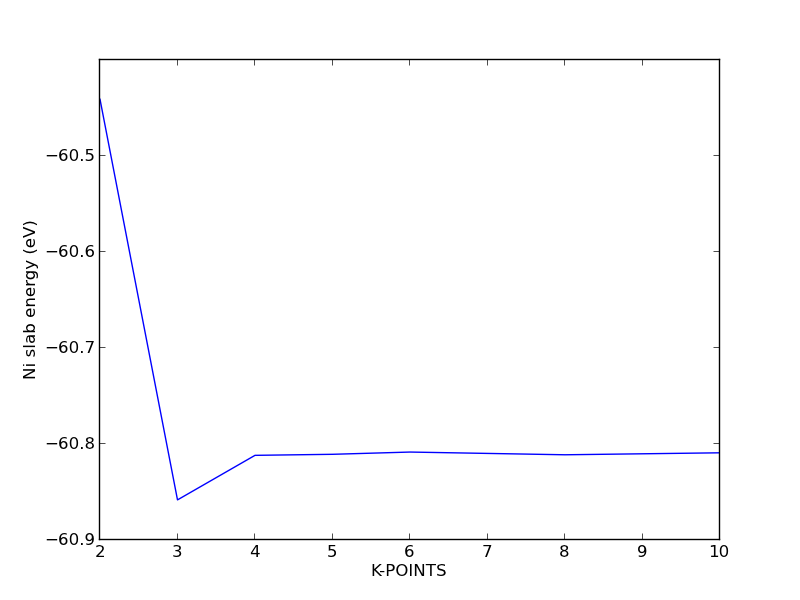
\includegraphics[width=0.7\textwidth]{./images/convergence/Ni_kpoint_convergence.png}
\caption{Ni kpoint convergence}
\end{figure}

We choose kpoint = 4
\subsubsection{convergence conclusion}
\label{sec-3-2-3}

I made convergence test to all metals and had the following table.
\begin{table}[H]
\caption{Parameters determinded by convergence study}
\begin{center}
\begin{tabular}{llrrrrr}
            &  O2       &   Ni  &   Cu  &   Pd  &   Pt  &   Au  \\
\hline
 encut(eV)  &  450      &  400  &  400  &  450  &  400  &  400  \\
 kpoints    &  Default  &    4  &    6  &    6  &    4  &    6  \\
\end{tabular}
\end{center}
\end{table}


The complete codes can be found at \href{file:///home/yichuns/FinalProject/convergence-study.org}{./convergence-study.org}
\subsection{clean slab energy}
\label{sec-3-3}

I will take Ni as an example. The rest metals are similar.

\begin{minted}[frame=lines,fontsize=\scriptsize,linenos]{python}
from jasp import *
from ase.lattice.surface import fcc111
from ase.constraints import FixAtoms

Thickness = [3,4,5,6]
D=[]
ready=True
for t in Thickness:
  atoms = fcc111('Ni', size=(2, 2, t), vacuum=10.0)
  constraint = FixAtoms(mask=[True for atom in atoms])
  atoms.set_constraint(constraint)
  with jasp('surfaces/Ni-slab-{0}'.format(t),
          xc='PBE',
          kpts=(4,4,1),
          encut=400,
          atoms=atoms) as calc:
    try:
       slab_e = atoms.get_potential_energy()
    except (VaspSubmitted,VaspQueued):
       slab_e=None

    D.append(slab_e)
if not ready:
 import sys; sys.exit()

import matplotlib.pyplot as plt
plt.plot(Thickness,D)
plt.xlabel('Number of layers')
plt.ylabel('Ni slab energy (eV)')
plt.savefig('images/Ni/slab.png')
plt.show()
\end{minted}

\begin{verbatim}
 None
\end{verbatim}
\begin{figure}[H]
\centering
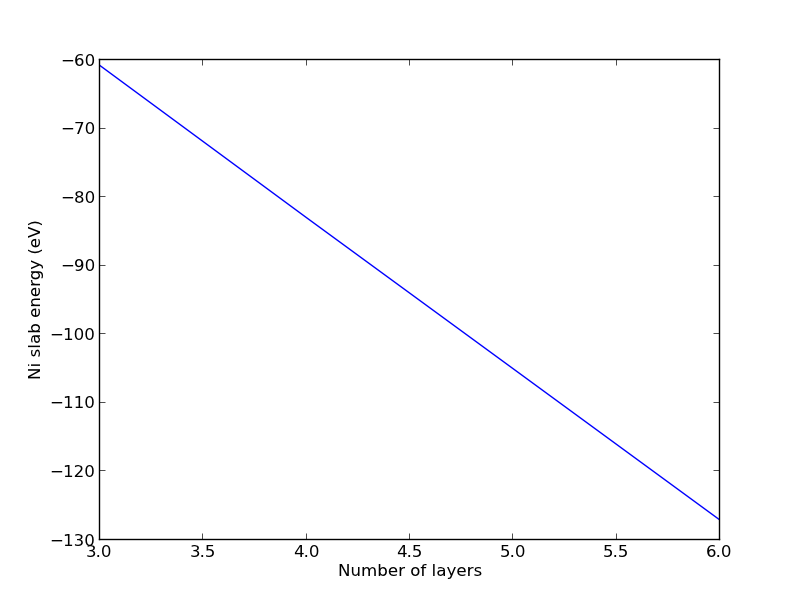
\includegraphics[width=0.7\textwidth]{./images/Ni/slab.png}
\caption{Ni clean slab energy of different layers}
\end{figure}
\subsection{slab + adsorbate energy}
\label{sec-3-4}
\subsubsection{fcc site}
\label{sec-3-4-1}


\begin{minted}[frame=lines,fontsize=\scriptsize,linenos]{python}
from jasp import *
from ase.lattice.surface import fcc111, add_adsorbate
from ase.constraints import FixAtoms

Thickness = [3,4,5,6]
add_e=[]
ready=True
for t in Thickness:
  atoms = fcc111('Ni', size=(2, 2, t), vacuum=10.0)

  add_adsorbate(atoms, 'O', height=1.2, position='fcc')

  constraint = FixAtoms(mask=[atom.symbol != 'O' for atom in atoms])
  atoms.set_constraint(constraint)

  with jasp('surfaces/Ni-slab-{0}-O-fcc'.format(t),
           xc='PBE',
           kpts=[4, 4, 1],
           encut=400,
           ibrion=2,
           nsw=25,
           atoms=atoms) as calc:
         try:
           calc.calculate()
           add_e.append(atoms.get_potential_energy())
         except (VaspSubmitted, VaspQueued):
           ready=False
if not ready:
 import sys; sys.exit()
import matplotlib.pyplot as plt
plt.plot(Thickness,add_e)
plt.xlabel('Layers of bulk')
plt.ylabel('Slab energy with addsorbate on (eV)')
plt.savefig('images/Ni/fcc-Slab-energy.png')
\end{minted}

\begin{verbatim}
 None
\end{verbatim}
\begin{figure}[H]
\centering
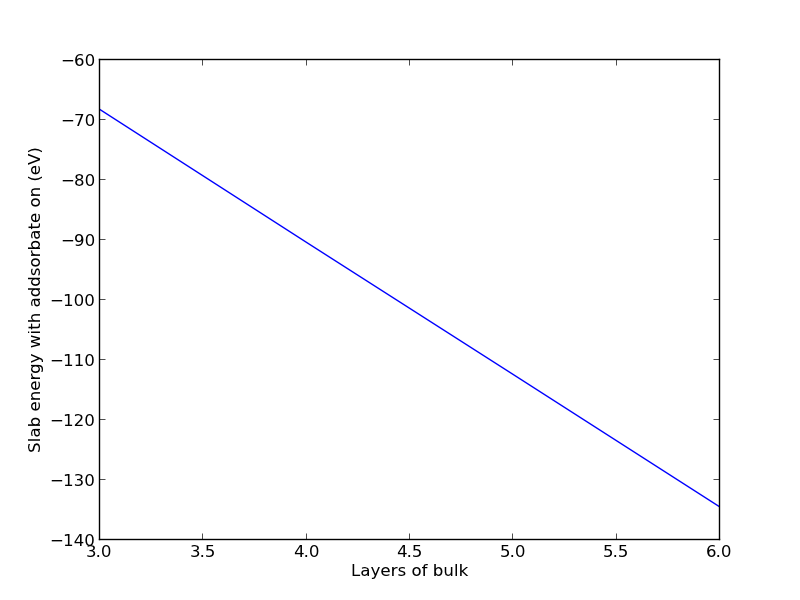
\includegraphics[width=0.7\textwidth]{./images/Ni/fcc-Slab-energy.png}
\caption{Ni fcc slab energy}
\end{figure}
\subsubsection{hcp site}
\label{sec-3-4-2}


\begin{minted}[frame=lines,fontsize=\scriptsize,linenos]{python}
from jasp import *
from ase.lattice.surface import fcc111, add_adsorbate
from ase.constraints import FixAtoms

Thickness = [3,4,5,6]
add_e=[]
ready=True
for t in Thickness:
  atoms = fcc111('Ni', size=(2, 2, t), vacuum=10.0)

  add_adsorbate(atoms, 'O', height=1.2, position='hcp')

  constraint = FixAtoms(mask=[atom.symbol != 'O' for atom in atoms])
  atoms.set_constraint(constraint)

  with jasp('surfaces/Ni-slab-{0}-O-hcp'.format(t),
           xc='PBE',
           kpts=[4, 4, 1],
           encut=400,
           ibrion=2,
           nsw=25,
           atoms=atoms) as calc:
         try:
           add_e.append(atoms.get_potential_energy())
         except (VaspSubmitted, VaspQueued):
           ready=False
if not ready:
 import sys; sys.exit()
import matplotlib.pyplot as plt
plt.plot(Thickness,add_e)
plt.xlabel('Layers of bulk')
plt.ylabel('Slab energy with addsorbate on (eV)')
plt.savefig('images/Ni/hcp-Slab-energy.png')
\end{minted}

\begin{verbatim}
 None
\end{verbatim}
\begin{figure}[H]
\centering
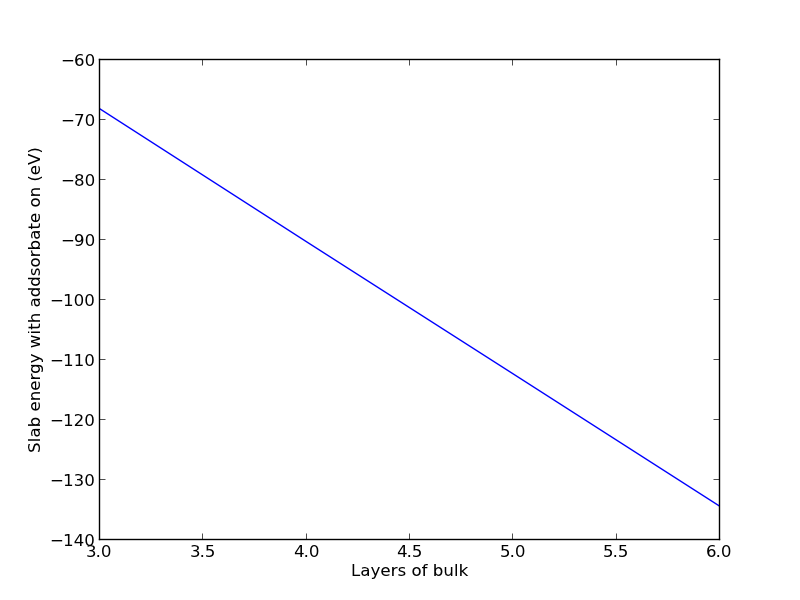
\includegraphics[width=0.7\textwidth]{./images/Ni/hcp-Slab-energy.png}
\caption{Ni hcp slab energy}
\end{figure}
\subsubsection{bridge site}
\label{sec-3-4-3}


\begin{minted}[frame=lines,fontsize=\scriptsize,linenos]{python}
from jasp import *
from ase.lattice.surface import fcc111, add_adsorbate
from ase.constraints import FixAtoms,FixScaled

Thickness = [3,4,5,6]
add_e=[]
ready=True
for t in Thickness:
  atoms = fcc111('Ni', size=(2, 2, t), vacuum=10.0)

  add_adsorbate(atoms, 'O', height=1.2, position='bridge')

  constraint1 = FixAtoms(mask=[atom.symbol != 'O' for atom in atoms])

  constraint2 = FixScaled(atoms.get_cell(),12 , [True, True, False])
  atoms.set_constraint([constraint1,constraint2])

  with jasp('surfaces/Ni-slab-{0}-O-bridge'.format(t),
           xc='PBE',
           kpts=[4, 4, 1],
           encut=400,
           ibrion=2,
           nsw=25,
           atoms=atoms) as calc:
         try:
           add_e.append(atoms.get_potential_energy())
         except (VaspSubmitted, VaspQueued):
           ready=False
if not ready:
 import sys; sys.exit()

import matplotlib.pyplot as plt
plt.plot(Thickness,add_e)
plt.xlabel('Layers of bulk')
plt.ylabel('Slab energy with addsorbate on (eV)')
plt.savefig('images/Ni/bridge-Slab-energy.png')
\end{minted}
\begin{verbatim}
 None
\end{verbatim}
\begin{figure}[H]
\centering
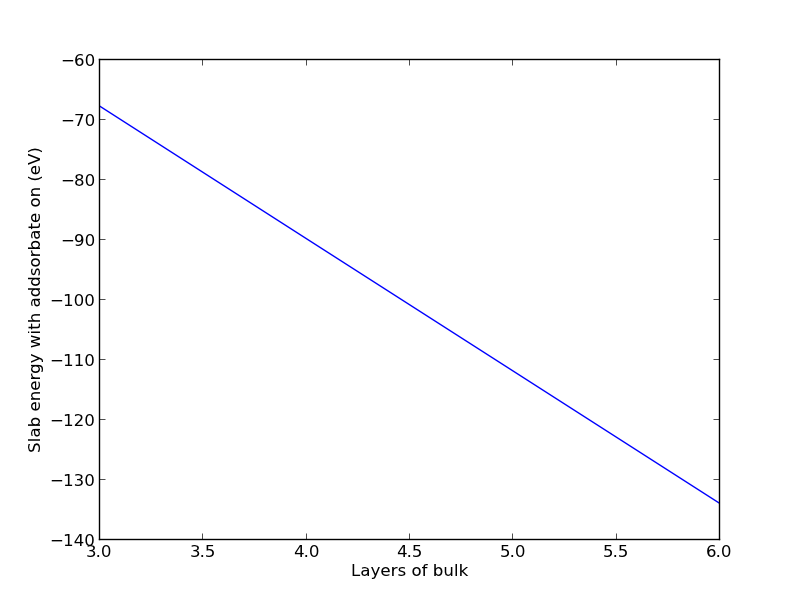
\includegraphics[width=0.7\textwidth]{./images/Ni/bridge-Slab-energy.png}
\caption{Ni bridge slab energy}
\end{figure}

The complete codes for all metals can be found at \href{file://../adsorption.org}{./adsorption.org}
\subsection{adsorption energy}
\label{sec-3-5}

Here I will take adsortion energy on fcc site of Ni as an example.

\begin{minted}[frame=lines,fontsize=\scriptsize,linenos]{python}
from jasp import *
import matplotlib.pyplot as plt
Thickness = [3,4,5,6]
Hads_fcc=[]
for t in Thickness:
 with jasp('surfaces/Ni-slab-{0}-O-fcc'.format(t)) as calc:
      atoms = calc.get_atoms()
      e_slab_o_fcc = atoms.get_potential_energy()

 with jasp('surfaces/Ni-slab-{0}'.format(t)) as calc:
      atoms = calc.get_atoms()
      e_slab = atoms.get_potential_energy()

 with jasp('convergence/O2/convergence-400') as calc:
      atoms = calc.get_atoms()
      e_O2 = atoms.get_potential_energy()

 Hads_fcc.append(e_slab_o_fcc - e_slab - 0.5*e_O2)

plt.plot(Thickness,Hads_fcc)
plt.xlabel('Number of layers')
plt.ylabel('Absorption energy of O2 on Ni (eV)')
plt.savefig('images/Ni/fcc-adsorption.png')
plt.show()
\end{minted}

\begin{verbatim}
 None
\end{verbatim}
\begin{figure}[H]
\centering
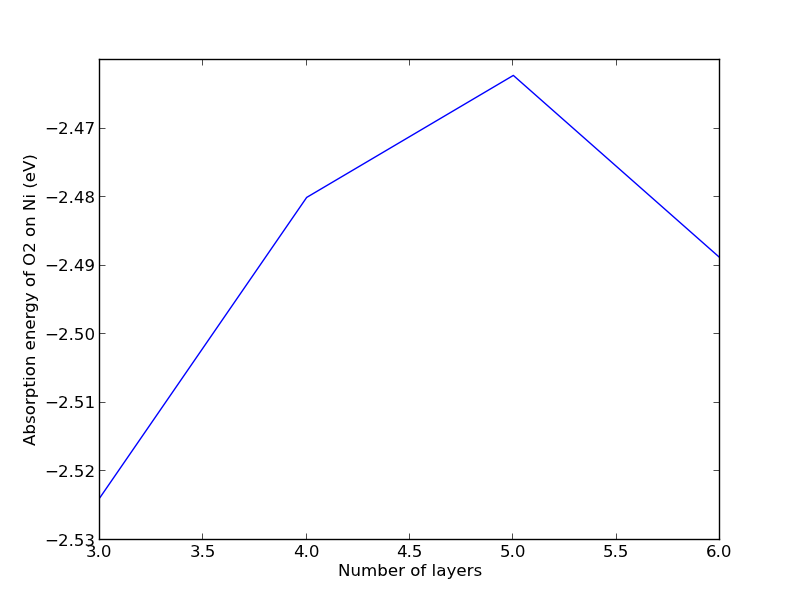
\includegraphics[width=0.7\textwidth]{./images/Ni/fcc-adsorption.png}
\caption{Ni fcc adsorption energy}
\end{figure}

The complete codes for all metals can be found at \href{file:///home/yichuns/FinalProject/Analysis.org}{./Analysis.org}
\section{Result and discussion}
\label{sec-4}


\begin{minted}[frame=lines,fontsize=\scriptsize,linenos]{python}
from jasp import *
import matplotlib.pyplot as plt
Thickness = [3,5,6]
elements=['Ni','Cu','Pt','Pd','Au']
plt.figure()

for e in elements:
 for t in Thickness:
  with jasp('surfaces/{1}-slab-{0}-O-fcc'.format(t,e)) as calc:
       atoms = calc.get_atoms()
       e_slab_o_fcc = atoms.get_potential_energy()

  with jasp('surfaces/{1}-slab-{0}-O-hcp'.format(t,e)) as calc:
       atoms = calc.get_atoms()
       e_slab_o_hcp = atoms.get_potential_energy()

  with jasp('surfaces/{1}-slab-{0}-O-bridge'.format(t,e)) as calc:
       atoms = calc.get_atoms()
       e_slab_o_bridge = atoms.get_potential_energy()

  with jasp('surfaces/{1}-slab-{0}'.format(t,e)) as calc:
       atoms = calc.get_atoms()
       e_slab = atoms.get_potential_energy()

  with jasp('convergence/O2/convergence-400') as calc:
       atoms = calc.get_atoms()
       e_O2 = atoms.get_potential_energy()

  Hads_fcc=e_slab_o_fcc - e_slab - 0.5*e_O2
  Hads_hcp=e_slab_o_hcp - e_slab - 0.5*e_O2
  Hads_bridge=e_slab_o_bridge - e_slab - 0.5*e_O2
  layer=[t,t,t]
  barrier=[Hads_fcc,Hads_bridge,Hads_hcp]
  print 'The fcc adsorption energy on {0} of {1} layers in {2:1.3f} eV'.format(e,t,Hads_fcc)
  print 'The hcp adsorption energy on {0} of {1} layers in {2:1.3f} eV'.format(e,t,Hads_hcp)
  print 'The bridge adsorption energy on {0} of {1} layers in {2:1.3f} eV'.format(e,t,Hads_bridge)
  plt.plot(layer,barrier,linestyle='none',marker='^')

plt.legend(elements,numpoints=1)
plt.xlim(2,7)
plt.xlabel('Number of layers')
plt.ylabel('Absorption energy of O2 on metals (eV)')

plt.savefig('images/result.png')

plt.show()
\end{minted}

\begin{verbatim}
 None
\end{verbatim}
\begin{figure}[H]
\centering
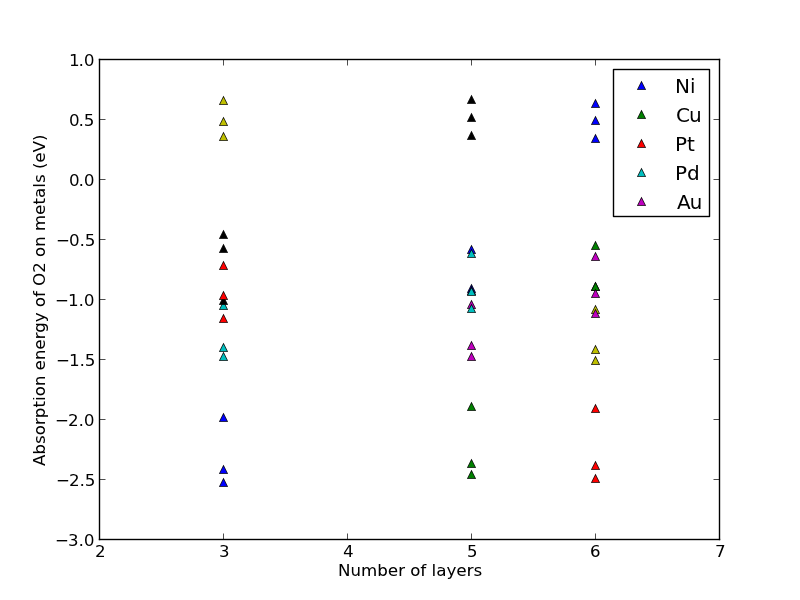
\includegraphics[width=0.7\textwidth]{./images/result.png}
\caption{Adsorption energy of O on different metals of different layers}
\end{figure}


\begin{verbatim}
The fcc adsorption energy on Ni of 3 layers in -2.524 eV
The hcp adsorption energy on Ni of 3 layers in -2.417 eV
The bridge adsorption energy on Ni of 3 layers in -1.982 eV
The fcc adsorption energy on Ni of 5 layers in -2.462 eV
The hcp adsorption energy on Ni of 5 layers in -2.367 eV
The bridge adsorption energy on Ni of 5 layers in -1.895 eV
The fcc adsorption energy on Ni of 6 layers in -2.489 eV
The hcp adsorption energy on Ni of 6 layers in -2.380 eV
The bridge adsorption energy on Ni of 6 layers in -1.909 eV
The fcc adsorption energy on Cu of 3 layers in -1.479 eV
The hcp adsorption energy on Cu of 3 layers in -1.397 eV
The bridge adsorption energy on Cu of 3 layers in -1.048 eV
The fcc adsorption energy on Cu of 5 layers in -1.475 eV
The hcp adsorption energy on Cu of 5 layers in -1.385 eV
The bridge adsorption energy on Cu of 5 layers in -1.040 eV
The fcc adsorption energy on Cu of 6 layers in -1.510 eV
The hcp adsorption energy on Cu of 6 layers in -1.421 eV
The bridge adsorption energy on Cu of 6 layers in -1.083 eV
The fcc adsorption energy on Pt of 3 layers in -1.009 eV
The hcp adsorption energy on Pt of 3 layers in -0.574 eV
The bridge adsorption energy on Pt of 3 layers in -0.461 eV
The fcc adsorption energy on Pt of 5 layers in -0.912 eV
The hcp adsorption energy on Pt of 5 layers in -0.580 eV
The bridge adsorption energy on Pt of 5 layers in -0.923 eV
The fcc adsorption energy on Pt of 6 layers in -0.892 eV
The hcp adsorption energy on Pt of 6 layers in -0.554 eV
The bridge adsorption energy on Pt of 6 layers in -0.892 eV
The fcc adsorption energy on Pd of 3 layers in -1.155 eV
The hcp adsorption energy on Pd of 3 layers in -0.966 eV
The bridge adsorption energy on Pd of 3 layers in -0.717 eV
The fcc adsorption energy on Pd of 5 layers in -1.075 eV
The hcp adsorption energy on Pd of 5 layers in -0.929 eV
The bridge adsorption energy on Pd of 5 layers in -0.619 eV
The fcc adsorption energy on Pd of 6 layers in -1.115 eV
The hcp adsorption energy on Pd of 6 layers in -0.947 eV
The bridge adsorption energy on Pd of 6 layers in -0.642 eV
The fcc adsorption energy on Au of 3 layers in 0.359 eV
The hcp adsorption energy on Au of 3 layers in 0.487 eV
The bridge adsorption energy on Au of 3 layers in 0.662 eV
The fcc adsorption energy on Au of 5 layers in 0.365 eV
The hcp adsorption energy on Au of 5 layers in 0.517 eV
The bridge adsorption energy on Au of 5 layers in 0.666 eV
The fcc adsorption energy on Au of 6 layers in 0.338 eV
The hcp adsorption energy on Au of 6 layers in 0.490 eV
The bridge adsorption energy on Au of 6 layers in 0.632 eV
\end{verbatim}

According to the low computational speed on layer 4(the reason is unknown), we will take layers 3,5,6 into consideration.It will not largely influence the conclusion. From the figure, we can see all adsorption energies are in the range of -3.0 eV and 1.0 eV. Most of them lie between -0.5 eV and -1.5 eV. Except for this, these data look like a mess. So I rearrange these data in a more understandable way.


\begin{minted}[frame=lines,fontsize=\scriptsize,linenos]{python}
from jasp import *
import matplotlib.pyplot as plt
Thickness = [3,5,6]
elements=['Ni','Cu','Pt','Pd','Au']
for t in Thickness:
 plt.figure()
 for e in elements:
  with jasp('surfaces/{1}-slab-{0}-O-fcc'.format(t,e)) as calc:
       atoms = calc.get_atoms()
       e_slab_o_fcc = atoms.get_potential_energy()

  with jasp('surfaces/{1}-slab-{0}-O-hcp'.format(t,e)) as calc:
       atoms = calc.get_atoms()
       e_slab_o_hcp = atoms.get_potential_energy()

  with jasp('surfaces/{1}-slab-{0}-O-bridge'.format(t,e)) as calc:
       atoms = calc.get_atoms()
       e_slab_o_bridge = atoms.get_potential_energy()

  with jasp('surfaces/{1}-slab-{0}'.format(t,e)) as calc:
       atoms = calc.get_atoms()
       e_slab = atoms.get_potential_energy()

  with jasp('convergence/O2/convergence-400') as calc:
       atoms = calc.get_atoms()
       e_O2 = atoms.get_potential_energy()

  Hads_fcc=e_slab_o_fcc - e_slab - 0.5*e_O2
  Hads_hcp=e_slab_o_hcp - e_slab - 0.5*e_O2
  Hads_bridge=e_slab_o_bridge - e_slab - 0.5*e_O2
  x=[1,2,3]
  barrier=[Hads_fcc,Hads_bridge,Hads_hcp]
  print 'Energy barrier of {0} of {1} layers from fcc to hcp is {2:1.3f} eV, from hcp to fcc is {3:1.3f} eV\n'.
#format(e,t,Hads_bridge-Hads_fcc,Hads_bridge-Hads_hcp)
  plt.plot(x,barrier)

 plt.xlabel('Displacement of O')
 plt.ylabel('Absorption energy of O2 on metals (eV)')
 plt.title('Barrier on {0} layers of different metals'.format(t))
 plt.legend(elements)
 plt.savefig('images/barrier-{0}.png'.format(t))
\end{minted}

Energy barrier of Ni of 3 layers from fcc to hcp is 0.542 eV, from hcp to fcc is 0.435 eV

Energy barrier of Cu of 3 layers from fcc to hcp is 0.431 eV, from hcp to fcc is 0.350 eV

Energy barrier of Pt of 3 layers from fcc to hcp is 0.548 eV, from hcp to fcc is 0.113 eV

Energy barrier of Pd of 3 layers from fcc to hcp is 0.438 eV, from hcp to fcc is 0.250 eV

Energy barrier of Au of 3 layers from fcc to hcp is 0.303 eV, from hcp to fcc is 0.175 eV

Energy barrier of Ni of 5 layers from fcc to hcp is 0.567 eV, from hcp to fcc is 0.472 eV

Energy barrier of Cu of 5 layers from fcc to hcp is 0.436 eV, from hcp to fcc is 0.346 eV

Energy barrier of Pt of 5 layers from fcc to hcp is -0.011 eV, from hcp to fcc is -0.343 eV

Energy barrier of Pd of 5 layers from fcc to hcp is 0.456 eV, from hcp to fcc is 0.310 eV

Energy barrier of Au of 5 layers from fcc to hcp is 0.300 eV, from hcp to fcc is 0.149 eV

Energy barrier of Ni of 6 layers from fcc to hcp is 0.580 eV, from hcp to fcc is 0.472 eV

Energy barrier of Cu of 6 layers from fcc to hcp is 0.427 eV, from hcp to fcc is 0.337 eV

Energy barrier of Pt of 6 layers from fcc to hcp is -0.000 eV, from hcp to fcc is -0.338 eV

Energy barrier of Pd of 6 layers from fcc to hcp is 0.474 eV, from hcp to fcc is 0.305 eV

Energy barrier of Au of 6 layers from fcc to hcp is 0.294 eV, from hcp to fcc is 0.142 eV

\begin{figure}[H]
\centering
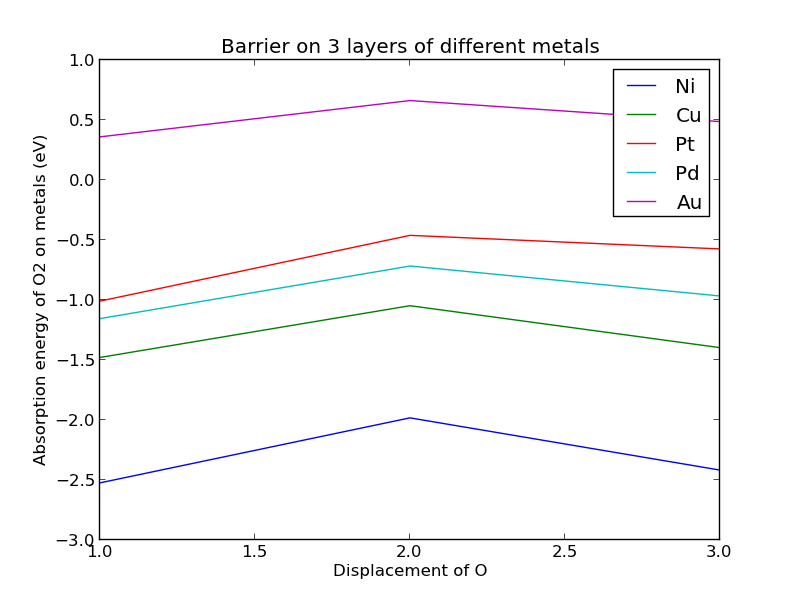
\includegraphics[width=0.7\textwidth]{./images/barrier-3.png}
\caption{Energy barriers of 3-layered metals}
\end{figure}

\begin{figure}[H]
\centering
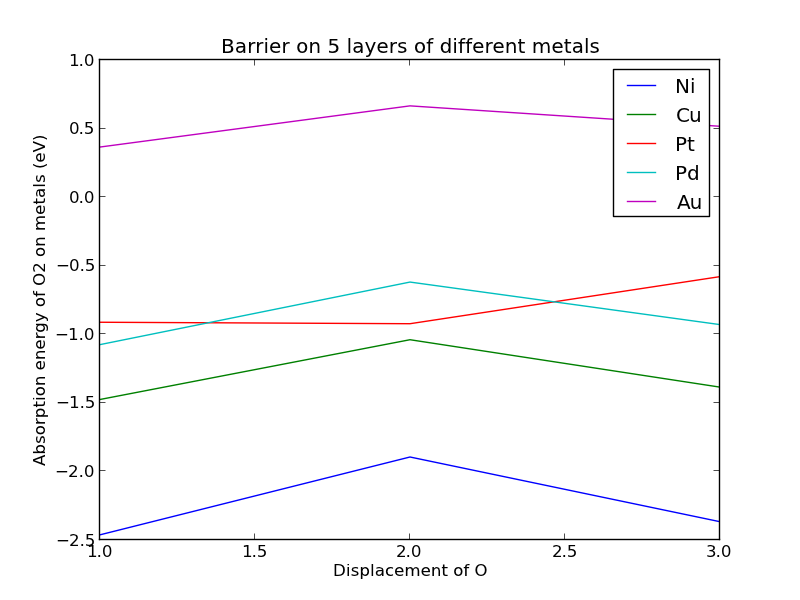
\includegraphics[width=0.7\textwidth]{./images/barrier-5.png}
\caption{Energy barriers of 5-layered metals}
\end{figure}

\begin{figure}[H]
\centering
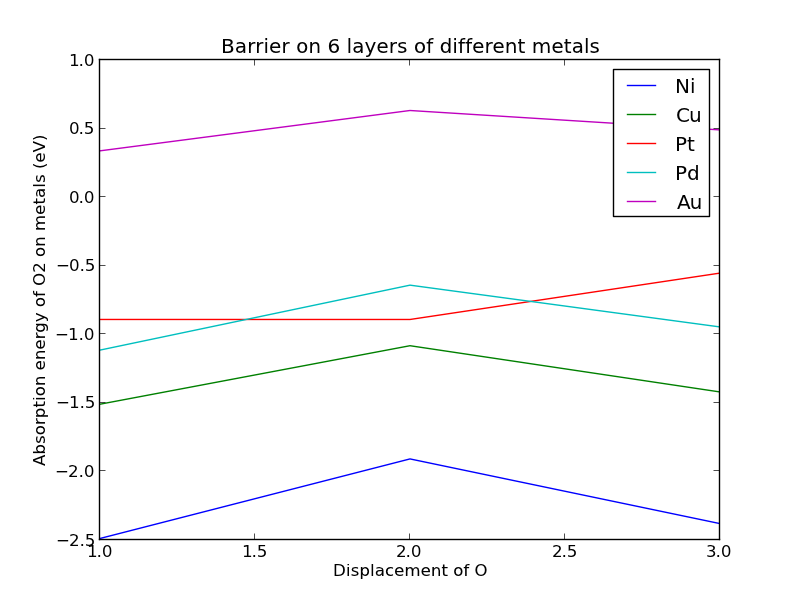
\includegraphics[width=0.7\textwidth]{./images/barrier-6.png}
\caption{Energy barriers of 6-layered metals}
\end{figure}

Interestingly, the barrier on Pt of 5 and 6 layers are totally different from 3 layer one. So I decided to put Pt aside for later analysis. Here I estimate the energy barrier of the rest metals of 3,5,6 layers.

\begin{table}[H]
\caption{Energy barrier from fcc to hcp}
\begin{center}
\begin{tabular}{lrrr}
 Number of layers  &      3  &      5  &      6  \\
\hline
 Ni (eV)           &  0.542  &  0.567  &  0.580  \\
 Cu (eV)           &  0.431  &  0.436  &  0.427  \\
 Pd (eV)           &  0.438  &  0.456  &  0.474  \\
 Au (eV)           &  0.303  &  0.300  &  0.294  \\
\end{tabular}
\end{center}
\end{table}


\begin{table}[H]
\caption{Energy barrier from hcp to fcc}
\begin{center}
\begin{tabular}{lrrr}
 Number of layers  &      3  &      5  &      6  \\
\hline
 Ni (eV)           &  0.435  &  0.472  &  0.472  \\
 Cu (eV)           &  0.350  &  0.346  &  0.337  \\
 Pd (eV)           &  0.250  &  0.310  &  0.305  \\
 Au (eV)           &  0.175  &  0.149  &  0.142  \\
\end{tabular}
\end{center}
\end{table}



From Table 2 and 3, we can see that the energy barrier from hcp to fcc is lower than that from fcc to hcp. It indicates that fcc site is the most stable site on surfaces of transition metals. Moreover, the barrier of Au lower than other metals. It implies that oxygen on Au surface will diffuse more freely than on other metal surfaces. This point explains why gold sometimes has more catalytic activity than other metal oxides.
\section{Conclusion}
\label{sec-5}

This project primarily has achieved the intial objective. In this project, I calculated the adsorption energies on five metals and estimated the diffusion barriers. The result shows that different adsorption energies, most of which are located  between -0.5 eV and -1.5 eV. For the diffusion barrier estimate, I find oxygen has the least resistance when diffusing on gold surface.
\subsection{Limitation}
\label{sec-5-1}

Here, when I found Pt's abnormal result, I checked the codes were right, comparing it to other metals. Then I checked the geometry of different sites on Pt.

\begin{figure}[H]
\centering
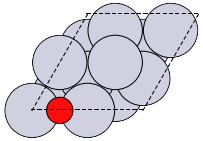
\includegraphics[width=203bp,]{./images/geometry/Pt-O-bridge-3.png}
\caption{Bridge site of 3-layered Pt}
\end{figure}

\begin{figure}[H]
\centering
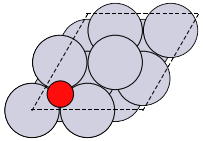
\includegraphics[width=203bp,]{./images/geometry/Pt-O-bridge-4.png}
\caption{Bridge site of 4-layered Pt}
\end{figure}

\begin{figure}[H]
\centering
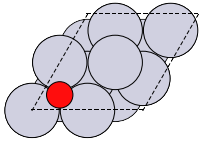
\includegraphics[width=203bp,]{./images/geometry/Pt-O-bridge-5.png}
\caption{Bridge site of 5-layered Pt}
\end{figure}

\begin{figure}[H]
\centering
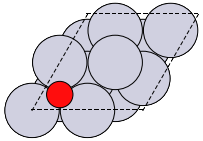
\includegraphics[width=203bp,]{./images/geometry/Pt-O-bridge-6.png}
\caption{Bridge site of 6-layered Pt}
\end{figure}

I found 3-layered Pt has a correct bridge site while the 4,5,6-layered all have fcc sites. This makes no sense and I still cannot find the bug.
\subsection{Future work}
\label{sec-5-2}

\begin{enumerate}
\item Because of the low computational speed, the 4-layered calculations are still running. So if this project add 4-layered data, it will be more complete and systematic.
\item When calculating the energy barrier, the method I used was a simple estimate. A more scientific approach is climbing NEB method. Thus, if this project is given more time, the climbing NEB method should be used in the calculation of energy barriers.
\end{enumerate}

\end{document}
